% !TEX root = ../thesis.tex
% basics
% @author Tobias Wulf
%

\chapter{Grundlagen 0.0.2 19.02.2021}\label{ch:grundlagen}
	\begin{itemize}
		\item Einleitung Aufgabenfeld
		\item Einheitskreis
		\item Bezug zur Drehwinkelerfassung und Sensorapplikation
	\end{itemize}




\section{Magnetische Sensorentypen und mechatronische Anwendung}\label{sec:magnetische-sensorentypen}
	\begin{itemize}
		\item Die Technologie mit der ein Sensorkopf realisiert ist, klassifiziert in der Regel die Sensorbezeichnung. Anhänge in der Bezeichnung wie AMR oder TMR, geben somit Auskunft darüber welche Technologie für die Realisierung des Sensorkopfes die Grundlage bildet.
		\item Anwendungsfall Winkelmessung
		\item Aufbau Sensorbrücke TMR (Umriss aus Datenblatt)
		\item Ausblick TMR Drehzahlmessung und Strommessung
	\end{itemize}

\section{Kennfeldmethode zur Charakterisierung von Sensoren}\label{sec:kennfeldmethode-zur-charakterisierung}
	\begin{itemize}
		\item Überleitung von Sensorbrückenschaltung
		\item Messprinzip für das Erstellen der Sensorbrücken-Kennfelder
		\item Festlegung von Arbeitsbereich (Plateau TMR), Sättigung (KMZ60)
		\item Dimensionierung des Stimulus, Dipole Anregung
	\end{itemize}
	
	
	\clearpage
	\begin{figure}[tbph]
		\centering
		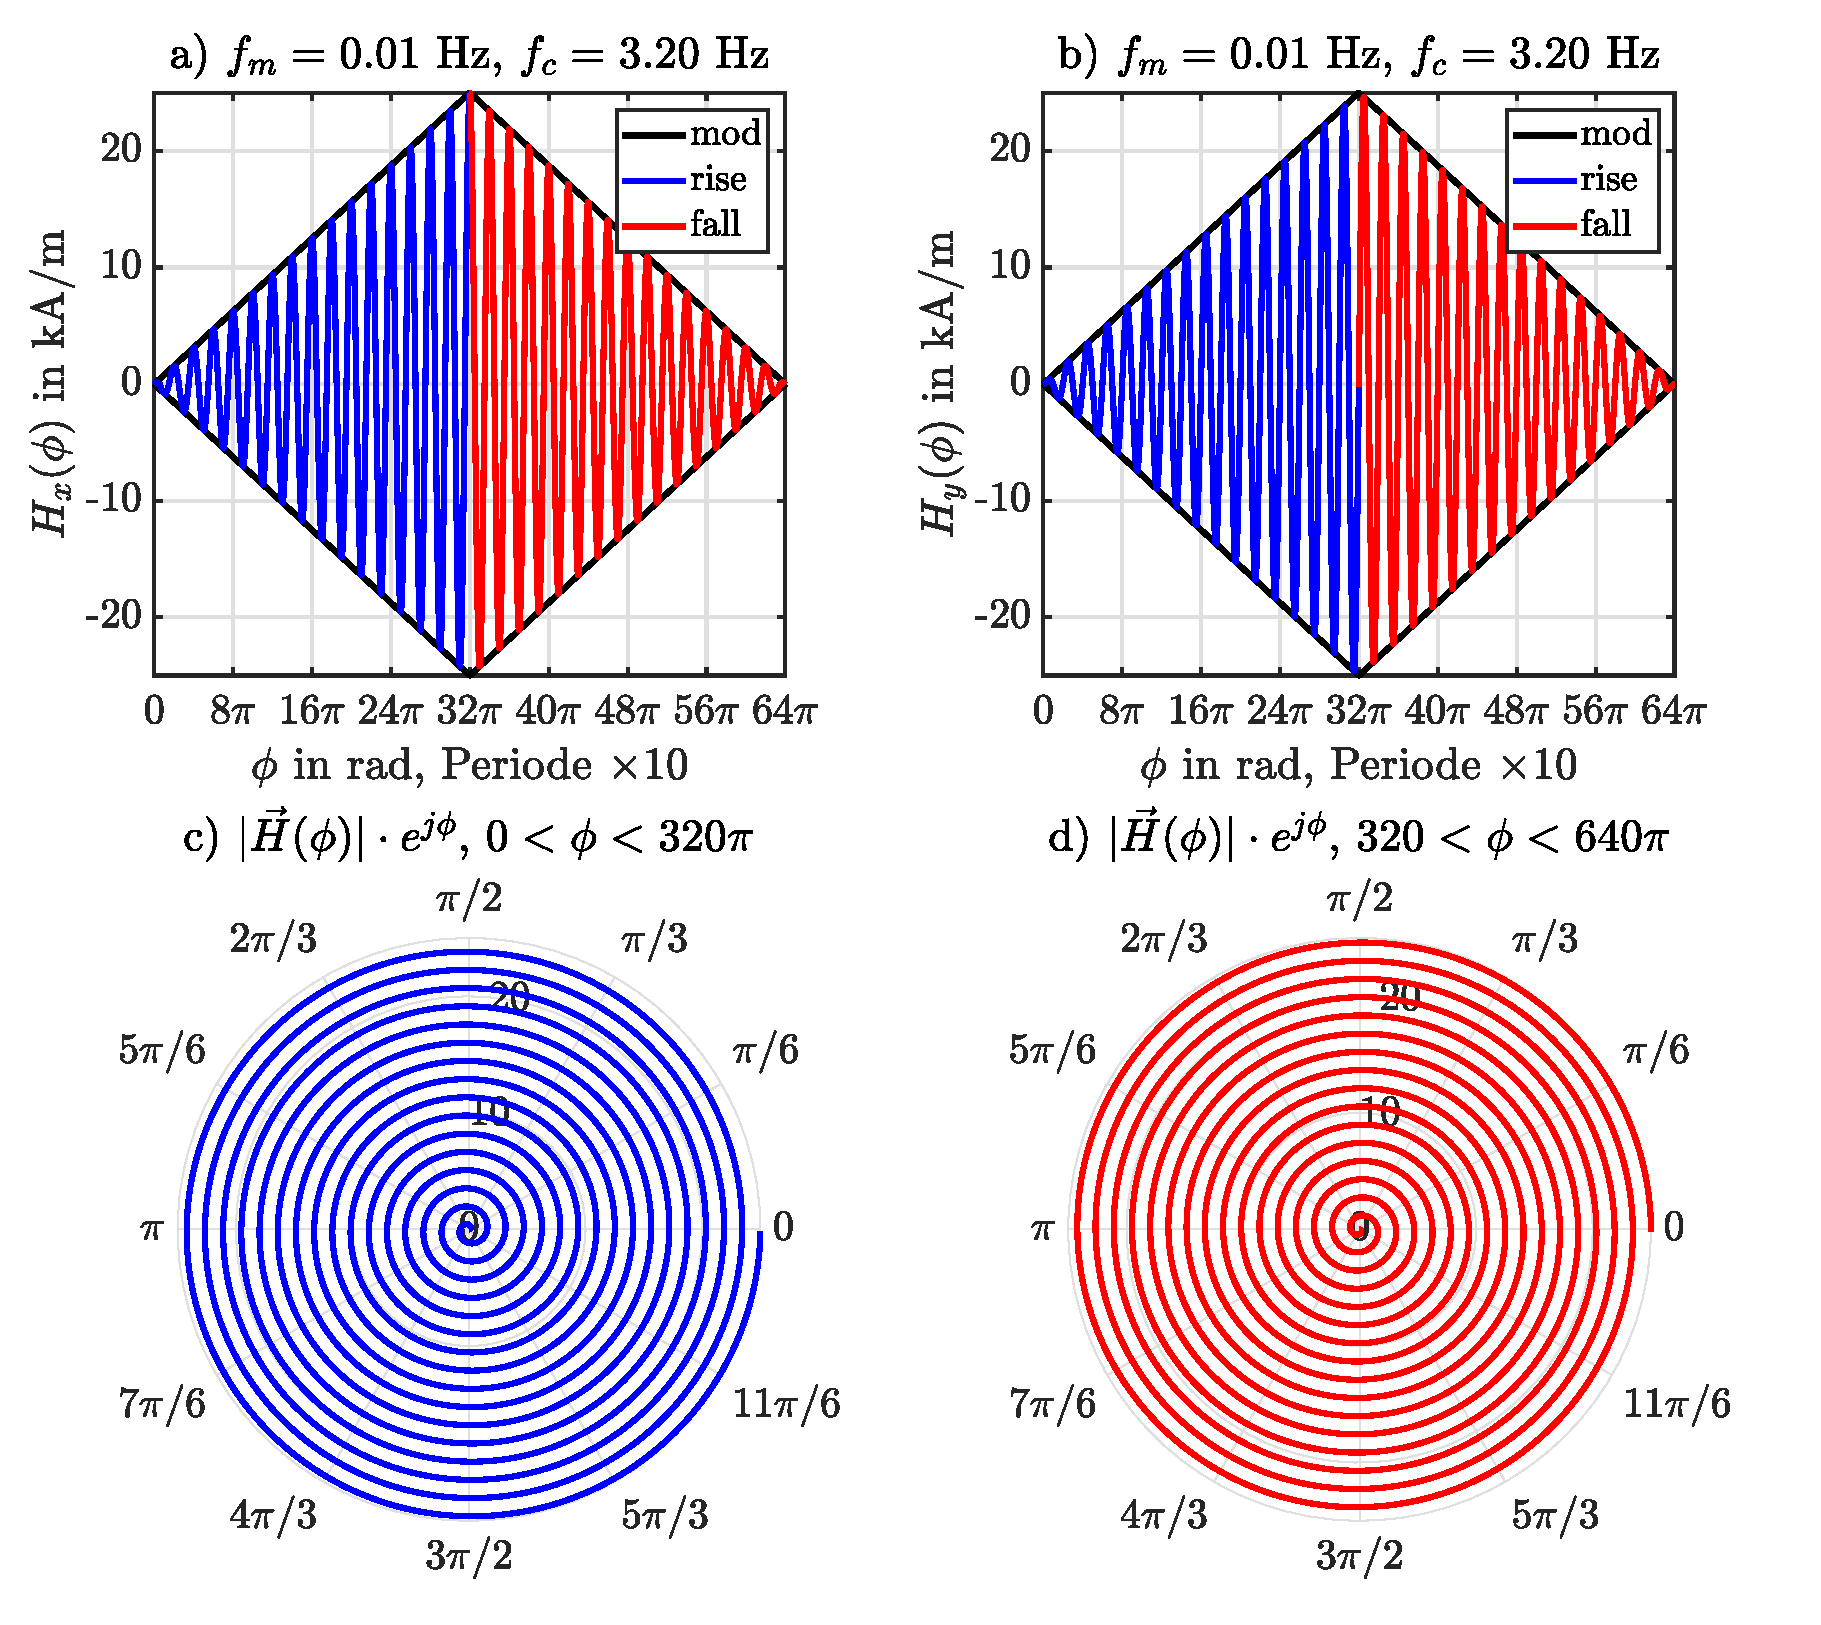
\includegraphics[width=\linewidth]{chapters/images/Magnetfeldstimulus_Kennfeldmethode}
		\caption[Magnetfeldstimulus zur Erzeugung von Sensorkennfeldern]{Magnetfeldstimulus zur Erzeugung von 
		Sensorkennfeldern. Es sind die Bestandteile des magnetischen Sensorstimuli dargestellt, die zum Ausmessen des 
		Sensorkennfeldes in $H_x$- und $H_y$-Richtung verwendet worden sind. Es ist das Prinzip des Verfahrens 
		dargestellt. In a) und b) ist die Dreiecksmodulation des magnetischen Anregungsfeldes abgebildet. Für a) die 
		$H_x$-Feldanregung mit Cosinus-Trägerwelle und für b) die $H_y$-Feldanregung mit Sinus-Trägerwelle. Es sind für 
		beide Anregungsrichtungen niedrige Frequenzen gewählt um ein quasi-statisches Anregungsmagnetfeld zu erzeugen. 
		Es ergeben sich für die Betragsamplitude des Stimulus, in polarer Darstellung c) und d), konzentrische 
		Trajektorien. Diese verlaufen von Innen nach Außen für die steigende Flanke der Amplitudenmodulation c) und von 
		Außen nach Innen für die fallende Flanke d). Die Dreieckmodulationsfrequenz liegt bei $f_m = \SI{0.1}{\hertz}$ 
		und einer Trägerwellenfrequenz $f_c = \SI{3.2}{\hertz}$.}
		\label{fig:magnetfeldstimuluskennfeldmethode}
	\end{figure}
	
	
	\clearpage
	\begin{figure}
		\centering
		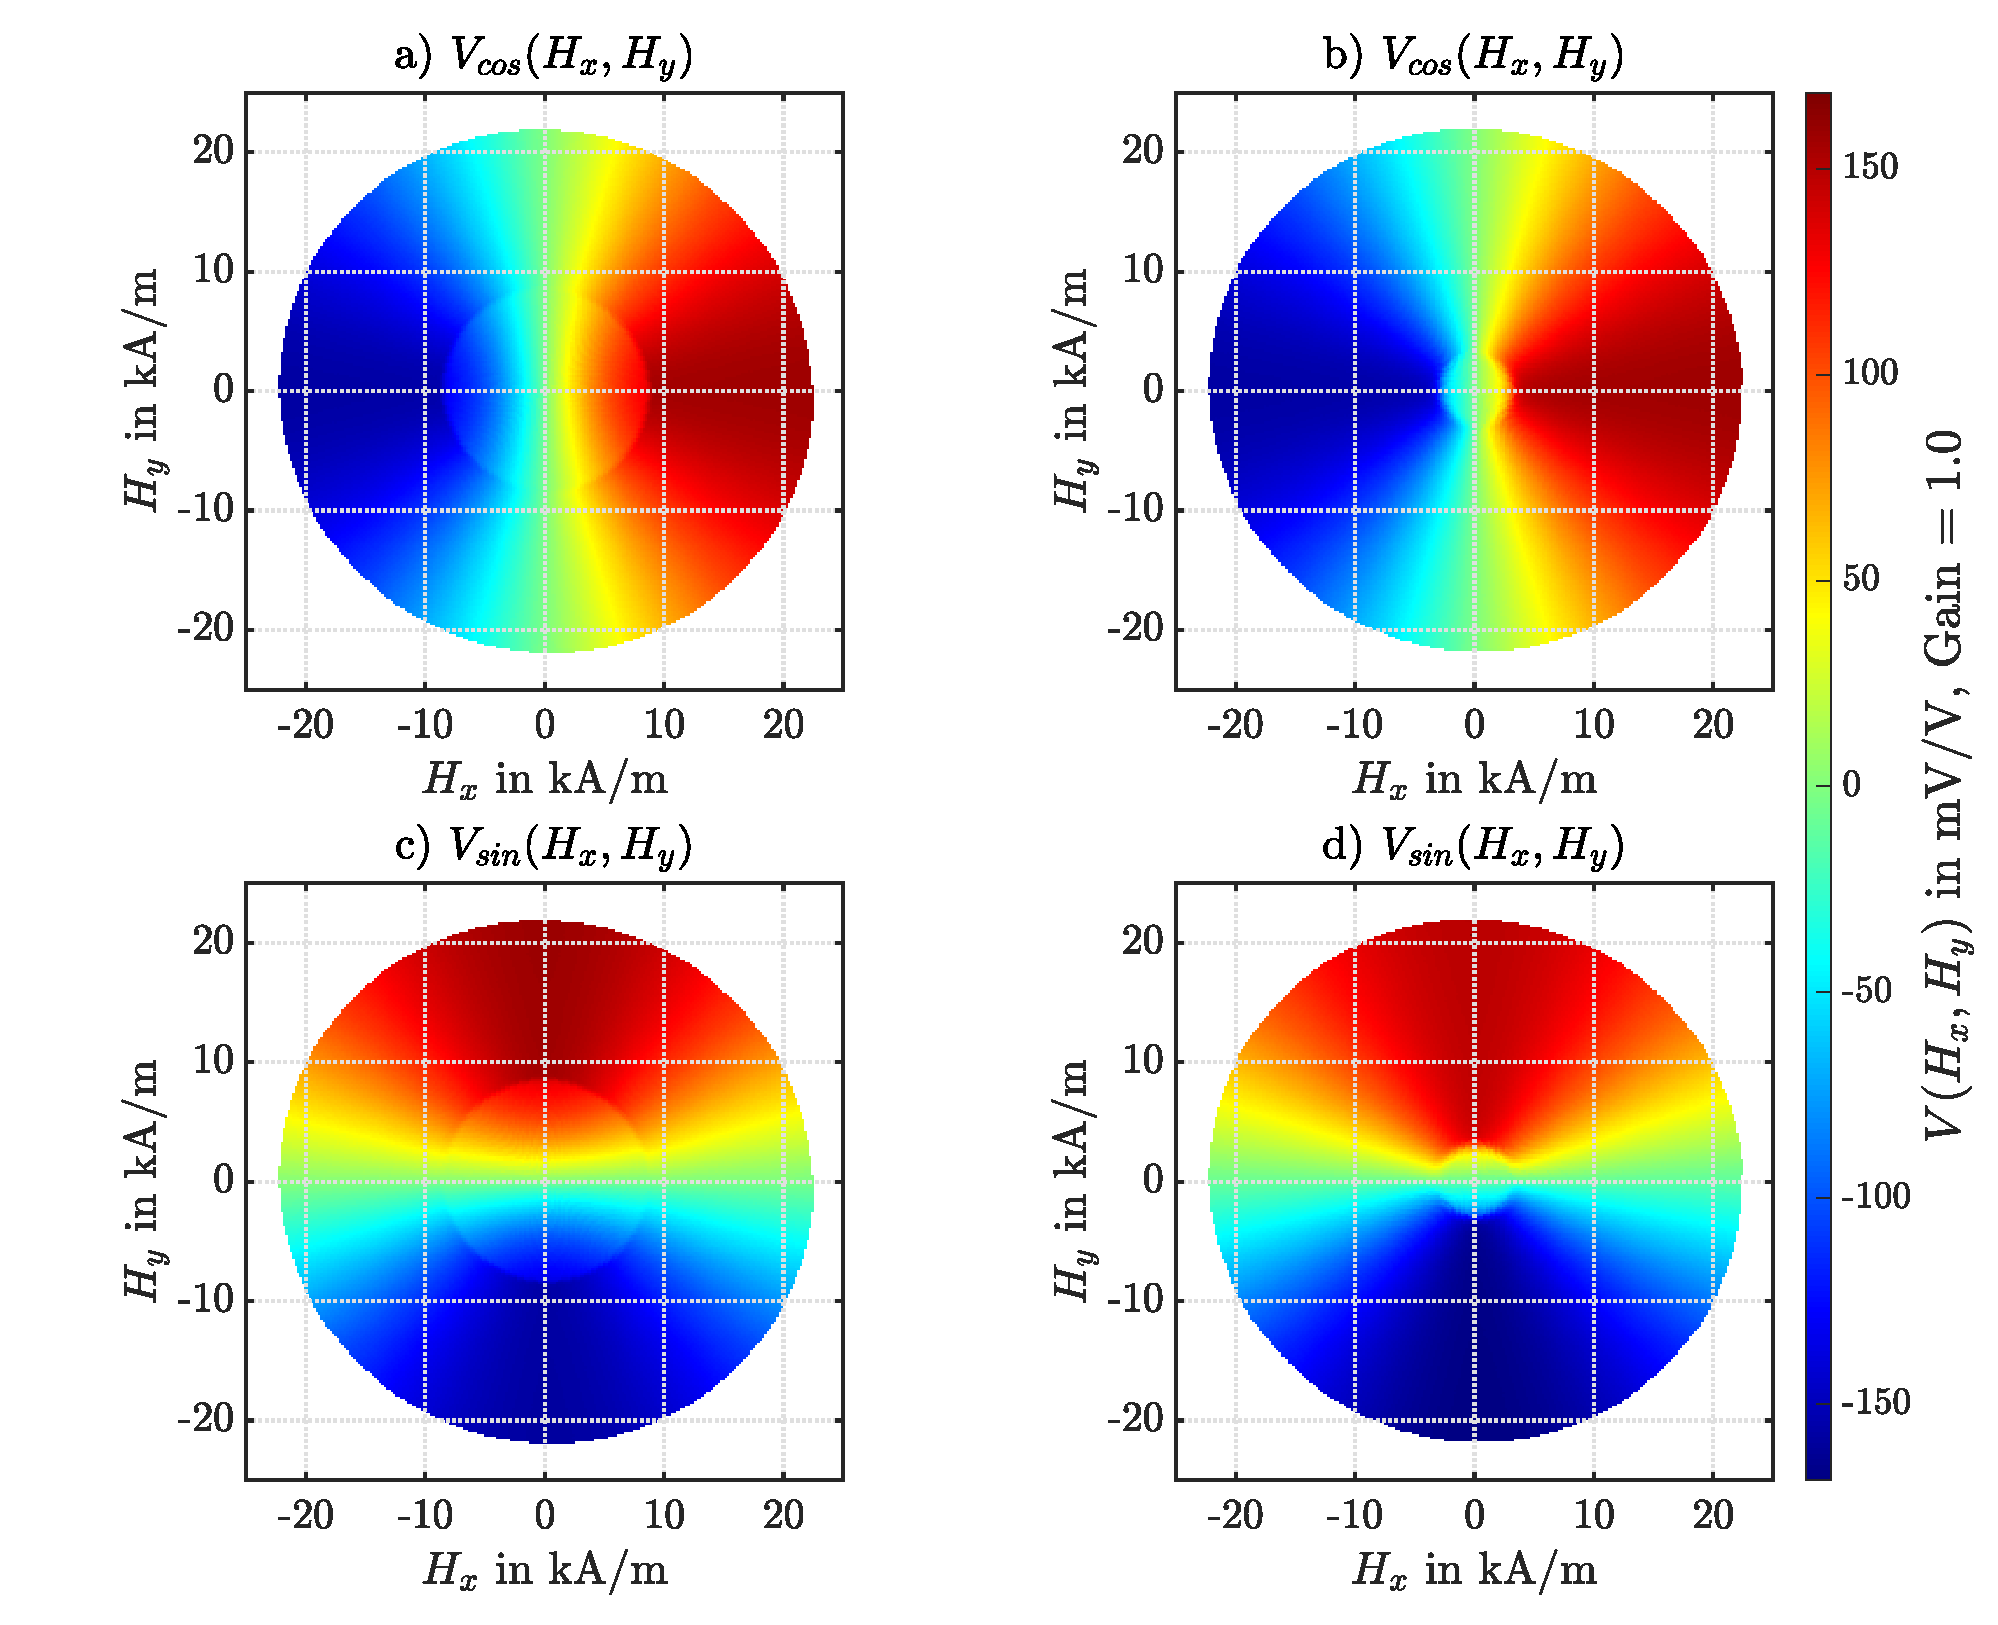
\includegraphics[width=\linewidth]{chapters/images/TDK_Kennfelder}
		\caption[TDK TAS2141-AAAB Winkelsensorbrückenkennfelder]{TDK TAS2141-AAAB Winkelsensorbrückenkennfelder. Zu 
		sehen sind die Kennfelder der Cosinus-Brücke a) und b). Darunter befinden sich die Kennfelder der Sinus-Brücke 
		c) und d). Die Kennfelder für beide Brücken a) und c) beziehen sich auf die steigenden Flanke der 
		Amplitudenmodulation aus \autoref{fig:magnetfeldstimuluskennfeldmethode} und die in b) bzw. d) gezeigten 
		Kennfelder sind gewonnen aus der fallenden Flanke. Die Brückenkennfelder sind normiert in 
		$\SI{}{\milli\volt\per\volt}$. Für eine Spannungsausgabe in Betriebsspannungsniveau ist keine zusätzliche 
		Verstärkung notwendig. Die Kennfelder besitzen, jeweils in $H_x$- und $H_y$-Richtung, eine Schrittweite von 
		$\SI{0.1961}{\kilo\ampere\per\metre}$ und sind skaliert von $\SI{-25}{\kilo\ampere\per\metre}$ bis 
		$\SI{+25}{\kilo\ampere\per\metre}$. Somit ergibt sich eine Bildauflösung für ein Kennfeld von $256 \times 256$ 
		Messpunkten.}
		\label{fig:tdkkennfelder}
	\end{figure}
	
	
	\clearpage
	\begin{figure}[tbph]
		\centering
		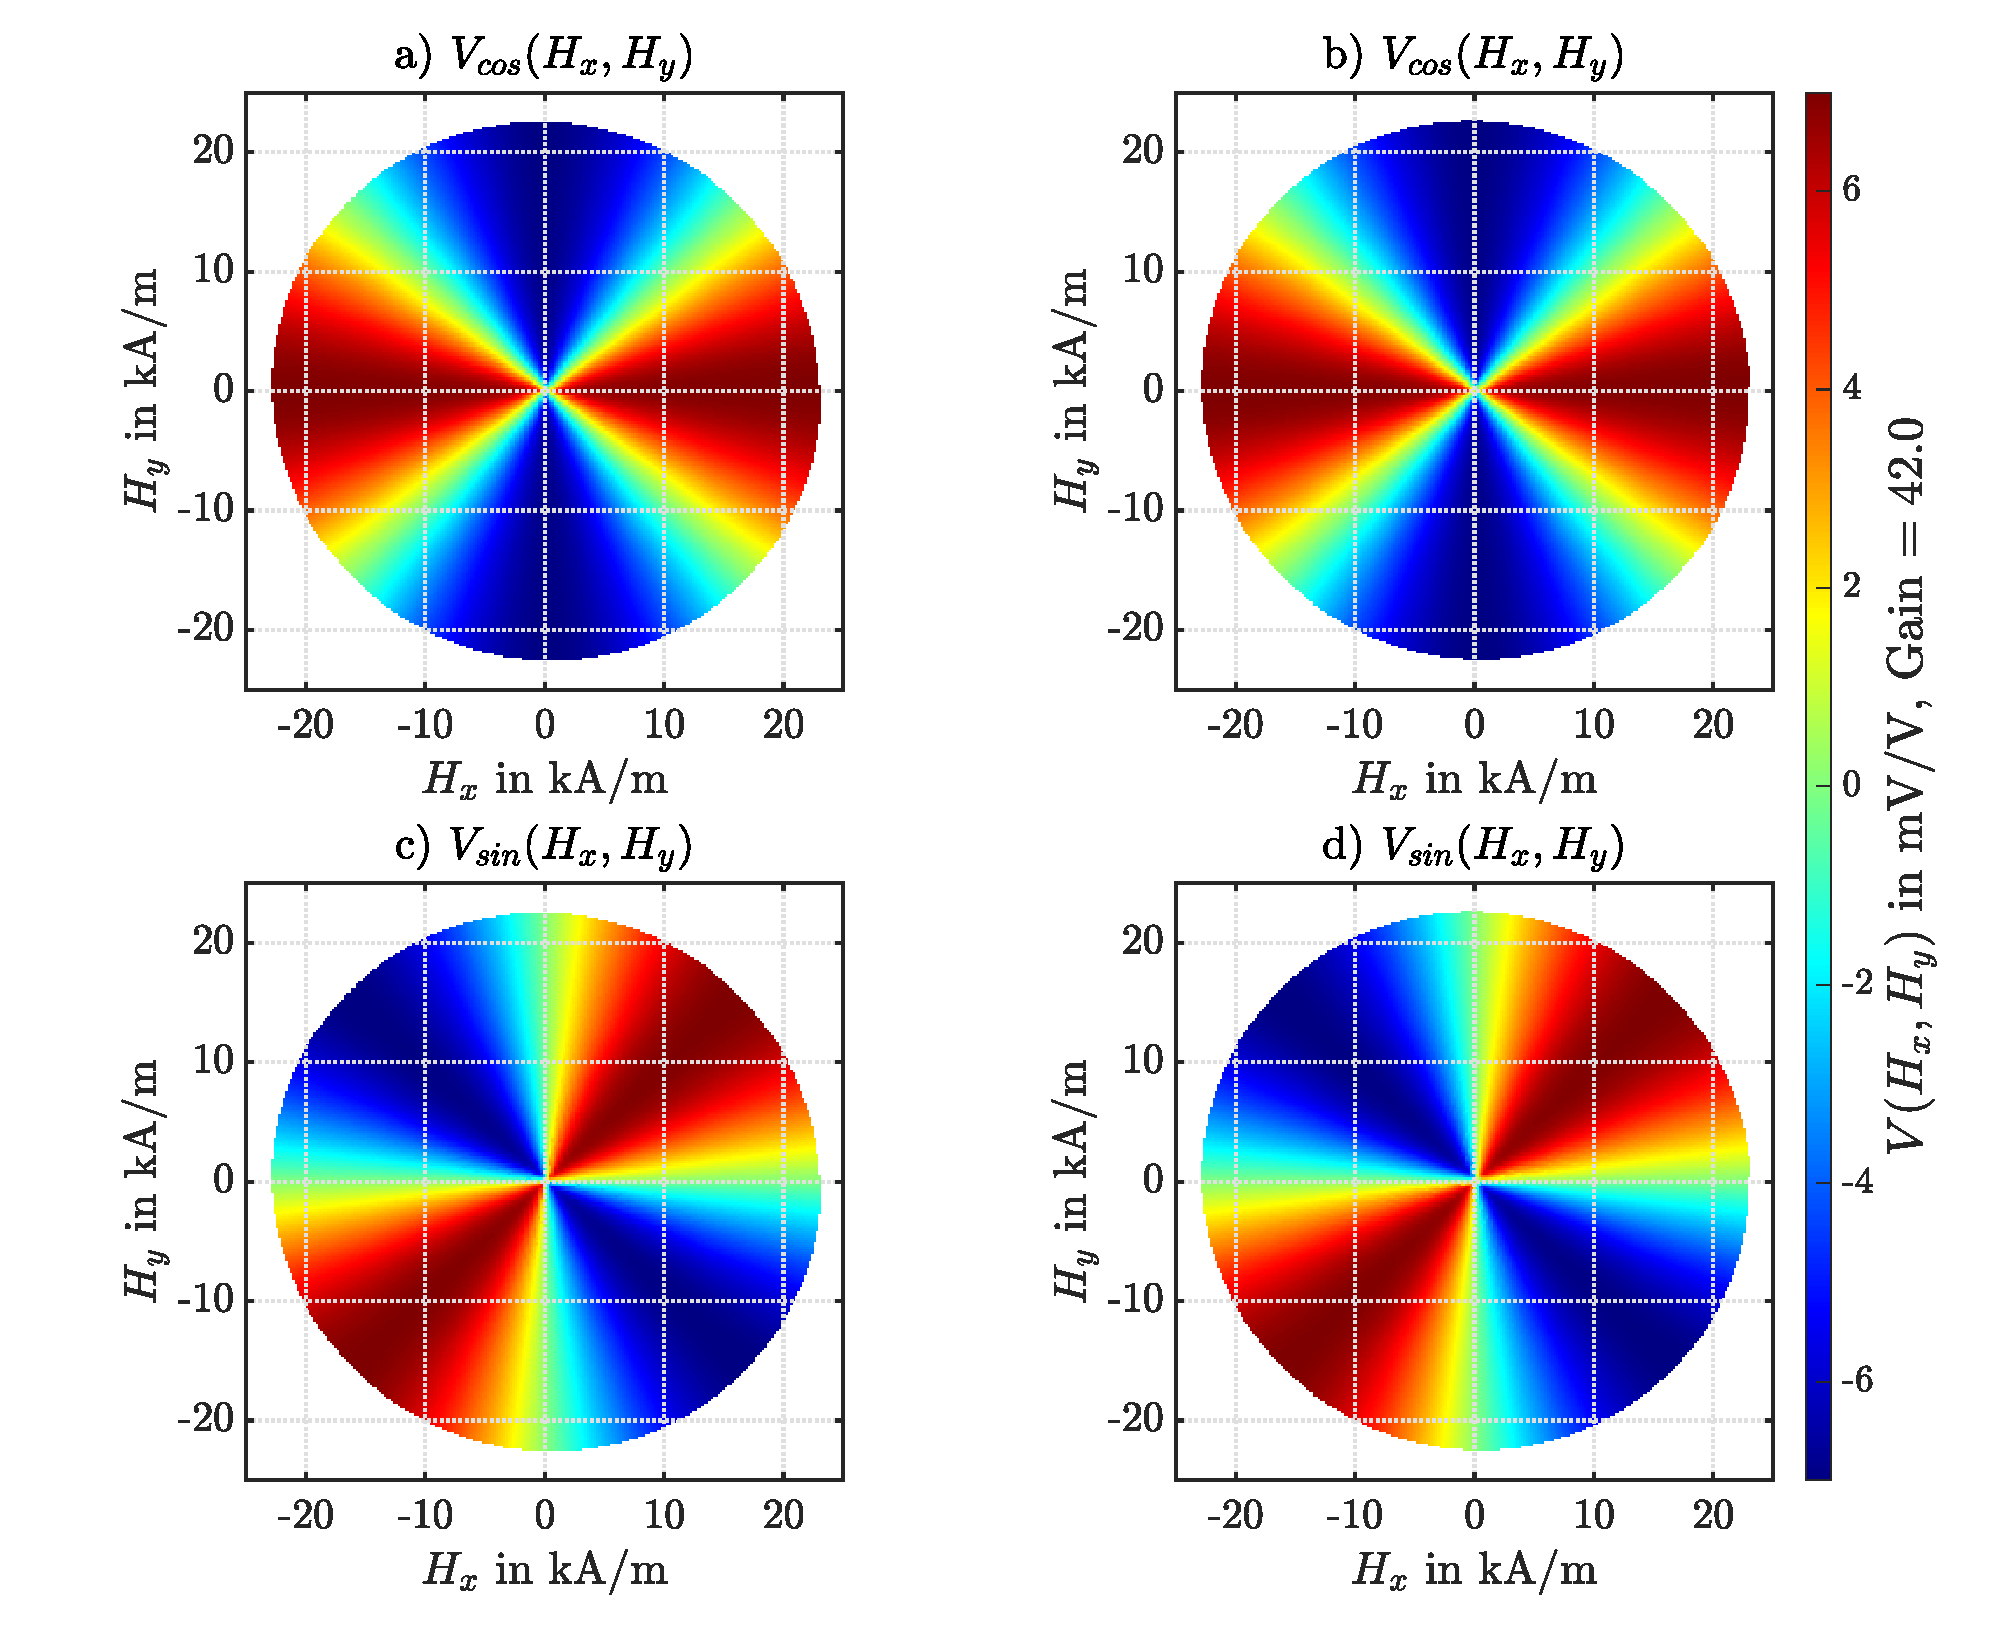
\includegraphics[width=\linewidth]{chapters/images/KMZ60_Kennfelder}
		\caption[NXP KMZ60 Winkelsensorbrückenkennfelder]{NXP KMZ60 Winkelsensorbrückenkennfelder. Zu sehen sind die 
		Kennfelder der Cosinus-Brücke a) und b). Darunter befinden sich die Kennfelder der Sinus-Brücke c) und d). 
		Die Kennfelder für beide Brücken a) und c) beziehen sich auf die steigenden Flanke der Amplitudenmodulation aus 
		\autoref{fig:magnetfeldstimuluskennfeldmethode} und die in b) bzw. d) gezeigten Kennfelder sind gewonnen aus 
		der fallenden Flanke. Die Brückenkennfelder sind normiert in $\SI{}{\milli\volt\per\volt}$. Für eine 
		Spannungsausgabe in Betriebsspannungsniveau ist eine zusätzliche Verstärkung um Faktor $42$ notwendig. Die 
		Kennfelder besitzen, jeweils in $H_x$- und $H_y$-Richtung, eine Schrittweite von 
		$\SI{0.1961}{\kilo\ampere\per\metre}$ und sind skaliert von $\SI{-25}{\kilo\ampere\per\metre}$ bis 
		$\SI{+25}{\kilo\ampere\per\metre}$. Somit ergibt sich eine Bildauflösung für ein Kennfeld von $256 \times 256$ 
		Messpunkten.}
		\label{fig:kmz60kennfelder}
	\end{figure}
	
	
	\clearpage
	\begin{figure}[tbph]
		\centering
		\includegraphics[width=\linewidth]{chapters/images/Approximierter_Kugelmagnet}
		\caption[Approximierter Kugelmagnet]{Approximierter Kugelmagnet. Die Approximation des Kugelmagneten erfolgt 
		über Dipol-Feldgleichung in Näherung des Kugelmagnetfernfeldes. Das Magnetfeld ist auf 
		$\SI{200}{\kilo\ampere\per\metre}$ bei einem Abstand von $\SI{1}{\milli\metre}$ zur Kugelmagnetoberfläche 
		normiert. Der Radius des Kugelmagneten beträgt $\SI{2}{\milli\metre}$.}
		\label{fig:dipolemagnet}
	\end{figure}
	
	
	\clearpage
	
	
\section{Prinzip des Sensor-Arrays}\label{sec:prinzip-des-sensor-arrays}
	\begin{itemize}
		\item geometrischer Aufbau
		\item Brückenausgangsspannungen
		\item Resultierende Array-Datenformate und Darstellung der Sinoiden
	\end{itemize}

\section{Sensor-Array-Simulation über Dipol-Feldgleichung}\label{sec:sensor-array-simulation-dipol-feldgleichung}
	\begin{itemize}
		\item Erzeugen des Meshgrids
		\item Normieren des Magnetfeldes
		\item Erzeugen von Rotationsmomenten (inkl. Verkippung)
		\item Referenzierung zu Kennfeldern und Gewinnung der Brückenspannungen (interp2 nearest neighbor)
	\end{itemize}

\section{Gauß-Prozesse für Regressionsverfahren}\label{sec:gauss-prozesse-regressionsverfahren}
	\begin{itemize}
		\item Erläuterung des Regressionsverfahren im allg.
		\item Bedeutung und Kriterien der Kovarianzfunktion, Spiegel der Applikation
		\item Herleitung der Quadratischen Frobenius Kovarianzfunktion mit Bezug zum Einheitskreis
		\item Möglichkeiten zur Mittelwertschätzung und -Korrektur
		\item Optimierungskriterien in der Trainingsphase
		\item Qualitätskriterien in der Arbeitsphase
	\end{itemize}